\documentclass{jlreq}

\usepackage{titlesec}
\usepackage{listings}
\usepackage{fancyhdr}

% url
\usepackage{url}

% \adjustbox
\usepackage{adjustbox}

% tcolorboxの設定
\usepackage[most]{tcolorbox} 
\tcbuselibrary{breakable}
\tcbuselibrary{skins}
\tcbuselibrary{listingsutf8}
% タイトルのフォーマットを変更
\titleformat{\title}
  {\centering\Huge\bfseries}
  {}
  {0em} 
  {}

\titleformat{\subtitle}
  {\centering\Large\itshape}
  {}
  {0em}
  {}

\titleformat{\subsubsection}[block]
  {\normalfont\normalsize\bfseries}
  {\arabic{subsubsection}.}
  {1em}
  {}

\titleformat{\section}[block]
  {\normalfont\large\bfseries}
  {\Roman{section}.}
  {1em} 
  {}
  [\titleline{\titlerule[1pt]}]

\titleformat{\subsection}[block]
  {\normalfont\normalsize\bfseries}
  {\roman{subsection}.}
  {1em}
  {}

% listingsの設定

\renewcommand{\lstlistingname}{コード}

\lstset{
	breaklines = true,
	language = Python,
	keywordstyle = {\bfseries \color[cmyk]{0,1,0,0}},
	commentstyle = {\itshape \color[cmyk]{1,0.4,1,0}},
	numbers = left,
	numberstyle = \tiny,
	stepnumber = 1,
	% frameとnumberの間の距離
	numbersep = 10pt,
	frame = single,
	basicstyle = \ttfamily,
	tabsize = 2,
	captionpos = t,
	backgroundcolor={\color[gray]{.90}},
	showstringspaces = false,
}

% headerの設定
\pagestyle{fancy}
\fancyhf{}

\fancyhead[RO,RE]{\rightmark}
\fancyhead[LO,LE]{\leftmark} 
\fancyfoot[C]{\thepage}

% tikzの設定
\usepackage{tikz}

\usepackage{amssymb} 

\newtcolorbox{definitionbox}[1][]{
    enhanced,
    title=#1, 
    attach boxed title to top left, 
    colback=white!95!blue,
    colbacktitle=white!10!blue!50!black,
    drop fuzzy shadow,
    boxrule=0.25mm,
}

% 定理環境
\newtcolorbox{theorembox}[1][]{
    enhanced,
    colback=white!95!green,
    colframe=green!40!black,
    coltitle=black,
    fonttitle=\bfseries,
    title=#1,
    attach boxed title to top left={yshift=-2mm, xshift=2mm},
    boxed title style={colback=green!30!white, size=small},
    drop fuzzy shadow,
    boxrule=0.5mm,
    sharp corners,
    top=4mm, bottom=4mm,
}


\begin{document} 
以下の章からは整数を扱います。

\section{最大公約数とユークリッドの互除法}

整数$a, b(a > b)$の最大公約数を求めるには、\textbf{ユークリッドの互除法}を使用します。

\begin{tcolorbox}[enhanced,title=ユークリッドの互除法, 
  attach boxed title to top left, 
  colback=white!95!blue,
  colbacktitle=white!10!blue!50!black,
  drop fuzzy shadow,
  boxrule=0.25mm,
  ]
  $a, b(a > b)$の最大公約数はa \% bとbの最大公約数と等しい。
\end{tcolorbox}

$a, b$の剰余を計算繰り返し計算していって$b$が0になった時の$a$が最大公約数となります。繰り返し同じ計算をするので、\textbf{再帰関数}
を使って実装します。

\begin{lstlisting}[caption=ユークリッドの互助法実装, frame=TRBL, label={euclid}]
def gcd(a: int, b: int) -> int:
  # 終了条件
  if b == 0:
      return a
  
  if a < b:
      a, b = b, a
      
  return gcd(b, a % b)
\end{lstlisting}

最大公約数をアルゴリズムを理解するだけではなくて、図形を使って直感的に理解しましょう。参考に記したけんちょんさんの最大公約数の記事を参考にすると、最大公約数は$n$次元の立方体を考えたときにそれを均等に分割できる最大の立方体の辺の長さとして考えることができます。このように考えると、最大公約数が何を意味しているのかが直感的に理解できるかもしれません。

\subsection{問題}
\subsubsection{ABC 118 C - Monsters Battle Royale}
問題からはすぐには気づきにくいですが、最大公約数を利用します。$n$次元の立方体を考えたときにそれを均等に分ける最大の立方体の辺の長さを求める問題と同じです。配列Aのどの要素もgcd
の倍数になっているので、gcdがこれ以上分割できない最小の辺の長さとなります。どんなに操作を加えても最小の辺の長さは変わりません。このように操作を繰り返しても
変わらない数のことを\textbf{不変量}といいます。与えられた配列Aの要素同士の引き算から必ずgcdを生み出せるかという疑問が生まれるかもしれませんが、
ユークリッドの互除法を使うことで、gcdを求めることができます。

\begin{tcolorbox}[enhanced, title=コラム 再帰関数, breakable, colback=white, drop fuzzy shadow, attach boxed title to top center={yshift*=0.1cm}]
  おそらく初めて再帰関数を見た方は再帰関数の動きがわかりにくいと思います。再帰関数は自分自身を呼び出す関数です。そのため、再帰関数を理解するためには、関数が呼び出された時にどのような動きをするのかを理解する必要があります。
  関数が呼び出されると、スタックに関数が積まれていきます。最初に呼び出したgcdは一番下に、最後に呼び出したgcdはスタックの一番上に置かれます。一番上の関数戻り値がわかったら、連鎖的にそれより下の関数の値もわかります。そして今回の場合シグネチャからもわかる通り、intのデータ型の値を返す関数です。
  returnする箇所で再びintの値を返す関数を呼び出しているので、スタックに積まれた関数がreturnするまで関数が呼び出され続けます。=が
  終了条件を満たすまで連なっていると考えるとわかりやすいかもしれません。
\end{tcolorbox}



\section{拡張ユークリッドの互除法}

ユークリッドの互除法では、最大公約数を求めることができますが、拡張ユークリッドの互除法を使うと、最大公約数だけでなく、$ax + by = \gcd(a, b)$を満たす$x, y$を求めることができます。

$ax + by = gcd(a, b)$の$a, b$に対してユークリッドの互除法を適用していきます。通常のユークリッドの互除法のように、$a \% b, b$を計算していきますが、計算した結果それがれが
次の一次不定方程式の係数となります。$b x_1 + \{(a\%b) y_1\} = gcd(a, b)$となります。ここで、

\begin{equation*}
    a \% b = a - (a//b) \times b
\end{equation*}

が成立することから、代入して

\begin{align*}
    b x_1 + ay_1 - (a//b) \times b y_1 = gcd(a, b) \\
    ay_1 + b(x_1 - (a//b) y_1) = gcd(a, b)
\end{align*}

$a x + b y = gcd(a, b)$と$a, b$について係数比較をすることで、

\begin{equation}
    x = y_1, y = x_1 - (a//b) \times y_1
\end{equation}


$x_1, y_1$は$b, a\%b$に対して再帰的に求めることができます。終了条件は$b = 0$のときで、このときの$x$が求める$x$となります。

具体例を見ましょう。$a = 108, b = 56$つまり$108 x + 56 y = gcd(108, 56)$です。

\begin{align*}
    108 x + 56 y &= gcd(108, 56) \\
    56 x_1 + 52 y_1 &= gcd(56, 52) \\
    52 x_2 + 4 y_2 &= gcd(52, 4) \\
    4 x_3 + 0 y_3 &= gcd(4, 0)
\end{align*}

$a x + by = gcd(a, b)$の解$(x, y)$が$b$と$a\%b$を係数にした一次不定方程式の解$(x_1, y_1)$から求められていることを確認してください。上から順に再帰的に(b, a\%b)を求めています。$b = 0$になったとき、$x_3 = 1, y_3 = 0$になります。式(1)より、
$x_2 = y_3 = 0, y_2 = x_3 - (52//4) \times y_3 = 1$となります。同様に、$x_1 = y_2 = 1, y_1 = x_2 - (56 // 54) y_2 = - 1$

以上より、$x = y_1 = -1, y = x_1 - (108 // 56) \times y_1$ = 2となります。

実装は以下のようになります。

\begin{lstlisting}[caption=拡張ユークリッドの互助法実装, frame=TRBL, label={euclid}]
def extended_gcd(a: int, b: int) -> tuple[int, int, int]:
    if b == 0:
        return a, 1, 0
    else:
        gcd, x1, y1 = extended_gcd(b, a % b)
    
        # 係数の更新
        x = y1
        y = x1 - (a // b) * y1
        
        return gcd, x, y
    

\end{lstlisting}

\subsection{参考}
\begin{itemize}
    \item \url{https://qiita.com/drken/items/0c88a37eec520f82b788}
\end{itemize}

\section{素数判定}

\subsection{ナイーブな実装}

ナイーブな実装では以下の定理を利用して、自然数$n$の素数判定を行います。

\begin{tcolorbox}[enhanced,title=定理1, 
  attach boxed title to top left, 
  colback=white!95!blue,
  colbacktitle=white!10!blue!50!black,
  drop fuzzy shadow,
  boxrule=0.25mm,
  ]
  自然数$n$が$\sqrt{n}$以下の素数で割り切れないならば、$n$は素数である。
\end{tcolorbox}
実装は以下のようになります。

\begin{lstlisting}[caption=ナイーブな素数判定, frame=TRBL, label={naivePriem}]
def is_prime(n: int) -> bool:
    # 忘れないように注意
    if n <= 1:
        return False
    i = 2
    while i * i <= n:
        if n % i == 0:
            return False
        i += 1
    
    return True

\end{lstlisting}

ナイーブな実装では、1個の自然数が素数か判定するには$O(\sqrt{n})$でできますが、$n$個の数を判定するとなったら$O(n \sqrt{n})$かかり少し遅いです。

\subsection{エラトステネスの篩}
多くの自然数の素数判定を高速に行う方法の1つに\textbf{エラトステネスの篩}があります。求める自然数の最大値を$n$とすると、
1から$n$までの自然数の素数判定はエラトステネスの篩を使うと、$O(n \log \log n)$の計算量で実行可能です。

エラトステネスのの篩では、判定したい自然数$n$までのテーブルを作成し、2から順に以下の操作を$\sqrt{n}$まで繰り返します。

\begin{enumerate}
  \item $i = 2$からスタート
  \item iがテーブルでバツがついていない場合、iを除いたiのすべての倍数を素数ではないとする
  \item $i = i + 1$ ($i = \sqrt{n}$まで2へ)
\end{enumerate}

例として$n = 100$の場合を見てみます。

\newpage


\begin{center}
  \begin{tabular}{|c|c|c|c|c|c|c|c|c|c|}
      \hline
      1  & 2  & 3  & 4  & 5  & 6  & 7  & 8  & 9  & 10 \\ \hline
      11 & 12 & 13 & 14 & 15 & 16 & 17 & 18 & 19 & 20 \\ \hline
      21 & 22 & 23 & 24 & 25 & 26 & 27 & 28 & 29 & 30 \\ \hline
      31 & 32 & 33 & 34 & 35 & 36 & 37 & 38 & 39 & 40 \\ \hline
      41 & 42 & 43 & 44 & 45 & 46 & 47 & 48 & 49 & 50 \\ \hline
      51 & 52 & 53 & 54 & 55 & 56 & 57 & 58 & 59 & 60 \\ \hline
      61 & 62 & 63 & 64 & 65 & 66 & 67 & 68 & 69 & 70 \\ \hline
      71 & 72 & 73 & 74 & 75 & 76 & 77 & 78 & 79 & 80 \\ \hline
      81 & 82 & 83 & 84 & 85 & 86 & 87 & 88 & 89 & 90 \\ \hline
      91 & 92 & 93 & 94 & 95 & 96 & 97 & 98 & 99 & 100 \\ \hline
  \end{tabular}

  \begin{tikzpicture}[overlay]
    % Loop for multiples of 2 (excluding 2 itself)
    \foreach \x in {3, 5, 7, 9, 11} {
        \foreach \y/\value in {5.84/2, 5.2/, 4.58/, 3.96/, 3.34/, 2.71/, 2.09/, 1.469/, 0.9/, 0.4/} {
            \ifnum\x=3\relax
                \ifdim\y pt=5.84pt \relax
                    % Skip the (2, 5.84) coordinate
                \else
                    \node at (-4.65+\x * 0.7, \y)[scale=2] {×};
                \fi
            \else
                \node at (-4.65+\x * 0.7, \y)[scale=2] {×};
            \fi
        }
    }
  \end{tikzpicture}
\end{center}
\vspace{0.1cm}


\begin{center}
    i = 2の場合
\end{center}

\vspace{0.5cm}

\begin{center}
  \begin{tabular}{|c|c|c|c|c|c|c|c|c|c|}
      \hline
      1  & 2  & 3  & 4  & 5  & 6  & 7  & 8  & 9  & 10 \\ \hline
      11 & 12 & 13 & 14 & 15 & 16 & 17 & 18 & 19 & 20 \\ \hline
      21 & 22 & 23 & 24 & 25 & 26 & 27 & 28 & 29 & 30 \\ \hline
      31 & 32 & 33 & 34 & 35 & 36 & 37 & 38 & 39 & 40 \\ \hline
      41 & 42 & 43 & 44 & 45 & 46 & 47 & 48 & 49 & 50 \\ \hline
      51 & 52 & 53 & 54 & 55 & 56 & 57 & 58 & 59 & 60 \\ \hline
      61 & 62 & 63 & 64 & 65 & 66 & 67 & 68 & 69 & 70 \\ \hline
      71 & 72 & 73 & 74 & 75 & 76 & 77 & 78 & 79 & 80 \\ \hline
      81 & 82 & 83 & 84 & 85 & 86 & 87 & 88 & 89 & 90 \\ \hline
      91 & 92 & 93 & 94 & 95 & 96 & 97 & 98 & 99 & 100 \\ \hline
  \end{tabular}

  \begin{tikzpicture}[overlay]
    % Loop for multiples of 2 (excluding 2 itself)
    \foreach \x in {3, 5, 7, 9, 11} {
        \foreach \y/\value in {5.84/2, 5.2/, 4.58/, 3.96/, 3.34/, 2.71/, 2.09/, 1.469/, 0.9/, 0.4/} {
            \ifnum\x=3\relax
                \ifdim\y pt=5.84pt \relax
                    % Skip the (2, 5.84) coordinate
                \else
                    \node at (-4.65+\x * 0.7, \y)[scale=2] {×};
                \fi
            \else
                \node at (-4.65+\x * 0.7, \y)[scale=2] {×};
            \fi
        }
    }

    % i = 3の場合を直打ち
    \node at (2.35, 5.84)[scale=2] {×}; % 9
    \node at (-0.4, 5.2)[scale=2] {×}; % 15
    \node at (-3.25, 4.58)[scale=2] {×}; % 21
    \node at (0.9,  4.58)[scale=2] {×}; % 27
    \node at (-1.85, 3.96)[scale=2] {×}; % 33
    \node at (2.35, 3.96)[scale=2] {×}; % 39
    \node at (-0.4, 3.34)[scale=2] {×}; % 45
    \node at (-3.25, 2.72)[scale=2] {×}; % 51
    \node at (0.9, 2.72)[scale=2] {×}; % 57
    \node at (-1.85, 2.09)[scale=2] {×}; % 63
    \node at (2.35, 2.09)[scale=2] {×}; % 69
    \node at (-0.4, 1.469)[scale=2] {×}; % 75
    \node at (-3.25, 0.9)[scale=2] {×}; % 81
    \node at (0.9, 0.9)[scale=2] {×}; % 87
    \node at (-1.85, 0.4)[scale=2] {×}; % 93
    \node at (2.35, 0.4)[scale=2] {×}; % 99


  \end{tikzpicture}
\end{center}


\begin{center}
    i = 3の場合
\end{center}

\vspace{0.5cm}


\begin{center}
    \begin{tabular}{|c|c|c|c|c|c|c|c|c|c|}
        \hline
        1  & 2  & 3  & 4  & 5  & 6  & 7  & 8  & 9  & 10 \\ \hline
        11 & 12 & 13 & 14 & 15 & 16 & 17 & 18 & 19 & 20 \\ \hline
        21 & 22 & 23 & 24 & 25 & 26 & 27 & 28 & 29 & 30 \\ \hline
        31 & 32 & 33 & 34 & 35 & 36 & 37 & 38 & 39 & 40 \\ \hline
        41 & 42 & 43 & 44 & 45 & 46 & 47 & 48 & 49 & 50 \\ \hline
        51 & 52 & 53 & 54 & 55 & 56 & 57 & 58 & 59 & 60 \\ \hline
        61 & 62 & 63 & 64 & 65 & 66 & 67 & 68 & 69 & 70 \\ \hline
        71 & 72 & 73 & 74 & 75 & 76 & 77 & 78 & 79 & 80 \\ \hline
        81 & 82 & 83 & 84 & 85 & 86 & 87 & 88 & 89 & 90 \\ \hline
        91 & 92 & 93 & 94 & 95 & 96 & 97 & 98 & 99 & 100 \\ \hline
    \end{tabular}
  
    \begin{tikzpicture}[overlay]
      % Loop for multiples of 2 (excluding 2 itself)
      \foreach \x in {3, 5, 7, 9, 11} {
          \foreach \y/\value in {5.84/2, 5.2/, 4.58/, 3.96/, 3.34/, 2.71/, 2.09/, 1.469/, 0.9/, 0.4/} {
              \ifnum\x=3\relax
                  \ifdim\y pt=5.84pt \relax
                      % Skip the (2, 5.84) coordinate
                  \else
                      \node at (-4.65+\x * 0.7, \y)[scale=2] {×};
                  \fi
              \else
                  \node at (-4.65+\x * 0.7, \y)[scale=2] {×};
              \fi
          }
      }
  
      % i = 3の場合を直打ち
      \node at (2.35, 5.84)[scale=2] {×}; % 9
      \node at (-0.4, 5.2)[scale=2] {×}; % 15
      \node at (-3.25, 4.58)[scale=2] {×}; % 21
      \node at (0.9,  4.58)[scale=2] {×}; % 27
      \node at (-1.85, 3.96)[scale=2] {×}; % 33
      \node at (2.35, 3.96)[scale=2] {×}; % 39
      \node at (-0.4, 3.34)[scale=2] {×}; % 45
      \node at (-3.25, 2.72)[scale=2] {×}; % 51
      \node at (0.9, 2.72)[scale=2] {×}; % 57
      \node at (-1.85, 2.09)[scale=2] {×}; % 63
      \node at (2.35, 2.09)[scale=2] {×}; % 69
      \node at (-0.4, 1.469)[scale=2] {×}; % 75
      \node at (-3.25, 0.9)[scale=2] {×}; % 81
      \node at (0.9, 0.9)[scale=2] {×}; % 87
      \node at (-1.85, 0.4)[scale=2] {×}; % 93
      \node at (2.35, 0.4)[scale=2] {×}; % 99

      % i = 5の場合を直打ち
      \node at (-0.4 ,4.55)[scale=2] {×}; % 25
        \node at (-0.4, 3.93)[scale=2] {×}; % 35
        \node at (-0.4, 2.72)[scale=2] {×}; % 55
        \node at (-0.4, 2.09)[scale=2] {×}; % 65
        \node at (-0.4, 0.9)[scale=2] {×}; % 85
        \node at (-0.4, 0.4)[scale=2] {×}; % 95
    \end{tikzpicture}
  \end{center}


  \begin{center}
    i = 5の場合
\end{center}

\vspace{0.5cm}

\begin{center}
    \begin{tabular}{|c|c|c|c|c|c|c|c|c|c|}
        \hline
        1  & 2  & 3  & 4  & 5  & 6  & 7  & 8  & 9  & 10 \\ \hline
        11 & 12 & 13 & 14 & 15 & 16 & 17 & 18 & 19 & 20 \\ \hline
        21 & 22 & 23 & 24 & 25 & 26 & 27 & 28 & 29 & 30 \\ \hline
        31 & 32 & 33 & 34 & 35 & 36 & 37 & 38 & 39 & 40 \\ \hline
        41 & 42 & 43 & 44 & 45 & 46 & 47 & 48 & 49 & 50 \\ \hline
        51 & 52 & 53 & 54 & 55 & 56 & 57 & 58 & 59 & 60 \\ \hline
        61 & 62 & 63 & 64 & 65 & 66 & 67 & 68 & 69 & 70 \\ \hline
        71 & 72 & 73 & 74 & 75 & 76 & 77 & 78 & 79 & 80 \\ \hline
        81 & 82 & 83 & 84 & 85 & 86 & 87 & 88 & 89 & 90 \\ \hline
        91 & 92 & 93 & 94 & 95 & 96 & 97 & 98 & 99 & 100 \\ \hline
    \end{tabular}
  
    \begin{tikzpicture}[overlay]
      % Loop for multiples of 2 (excluding 2 itself)
      \foreach \x in {3, 5, 7, 9, 11} {
          \foreach \y/\value in {5.84/2, 5.2/, 4.58/, 3.96/, 3.34/, 2.71/, 2.09/, 1.469/, 0.9/, 0.4/} {
              \ifnum\x=3\relax
                  \ifdim\y pt=5.84pt \relax
                      % Skip the (2, 5.84) coordinate
                  \else
                      \node at (-4.65+\x * 0.7, \y)[scale=2] {×};
                  \fi
              \else
                  \node at (-4.65+\x * 0.7, \y)[scale=2] {×};
              \fi
          }
      }
  
      % i = 3の場合を直打ち
      \node at (2.35, 5.84)[scale=2] {×}; % 9
      \node at (-0.4, 5.2)[scale=2] {×}; % 15
      \node at (-3.25, 4.58)[scale=2] {×}; % 21
      \node at (0.9,  4.58)[scale=2] {×}; % 27
      \node at (-1.85, 3.96)[scale=2] {×}; % 33
      \node at (2.35, 3.96)[scale=2] {×}; % 39
      \node at (-0.4, 3.34)[scale=2] {×}; % 45
      \node at (-3.25, 2.72)[scale=2] {×}; % 51
      \node at (0.9, 2.72)[scale=2] {×}; % 57
      \node at (-1.85, 2.09)[scale=2] {×}; % 63
      \node at (2.35, 2.09)[scale=2] {×}; % 69
      \node at (-0.4, 1.469)[scale=2] {×}; % 75
      \node at (-3.25, 0.9)[scale=2] {×}; % 81
      \node at (0.9, 0.9)[scale=2] {×}; % 87
      \node at (-1.85, 0.4)[scale=2] {×}; % 93
      \node at (2.35, 0.4)[scale=2] {×}; % 99

      % i = 5の場合を直打ち
      \node at (-0.4 ,4.55)[scale=2] {×}; % 25
        \node at (-0.4, 3.93)[scale=2] {×}; % 35
        \node at (-0.4, 2.72)[scale=2] {×}; % 55
        \node at (-0.4, 2.09)[scale=2] {×}; % 65
        \node at (-0.4, 0.9)[scale=2] {×}; % 85
        \node at (-0.4, 0.4)[scale=2] {×}; % 95
    
    
        % i = 7の場合を直打ち
        \node at (2.35, 3.34) [scale=2] {×}; % 49
        \node at (0.9, 1.469) [scale=2] {×}; % 77
        \node at (-3.25, 0.4) [scale=2] {×}; % 91
    \end{tikzpicture}
  \end{center}

\begin{center}
    i = 7の場合
\end{center}

1を除いて残った数が素数です。

\subsection{エラトステネスの篩の実装}

\begin{lstlisting}[caption=エラトステネスの篩の実装, label=stack, frame=TRBL]
def is_prime(n: int) -> list[bool]:
    is_prime_list = [True] * (n + 1)
    is_prime_list[0] = is_prime_list[1] = False
    i = 2
    while i * i <= n:
        if is_prime_list[i]:
            for j in range(i * i,n + 1,i):
                is_prime_list[j] = False
        i += 1

    return is_prime_list
\end{lstlisting}

\subsection{参考}

\begin{itemize}
    \item \url{https://algo-method.com/tasks/318}
\end{itemize}

\section{素因数分解}
\subsection{ナイーブな実装}

ナイーブな素因数分解では、与えられた自然数$n$を2から$\sqrt{n}$まで順に割っていき、1になれば終了します。割り切れた数を素因数としてリストに追加していきます。
$\sqrt{n}$まで続けて$n$が1でない場合は、その数も素因数としてリストに追加します。

\begin{lstlisting}[caption=ナイーブな素因数分解の実装の実装, label=factor, frame=TRBL]
def enumerate_prime_factors(n: int) -> list[int]:
    primes = []
    i = 2
    while i * i <= n:
        if n % i == 0:
            primes.append(i)
            n //= i
            while n % i == 0:
                primes.append(i)
                n //= i
        i += 1

    # 残ったnが素数の場合
    if n > 1:
        primes.append(int(n))

    return primes
\end{lstlisting}

ナイーブな実装では、自然数$n$が与えられたときの計算量は$O(\sqrt{n})$です。$m$個の素因数分解をするときは
計算量が$O(m \sqrt{n})$となります。 

\subsection{SPFを用いた実装}

SPF(Smallest Prime Factor: 自然数$n$を割り切る最小の素数)を用いることで、ナイーブな実装よりも高速に素因数分解を行うことができます。SPFを用いた素因数分解は
エラトステネスの篩をする際にSPFを記録することで実装できます。

\begin{lstlisting}[caption=SPFを用いた素因数分解の実装, label=spf, frame=TRBL]
def spf(n: int) -> list[int]:
        spf_table = [i for i in range(n + 1)]
        is_prime = [True] * (n + 1)
        
        i = 2
        
        while i * i <= n:
            if is_prime[i]:
                for j in range(i + i, n + 1, i):
                    is_prime[j] = False
                    if spf_table[j] == j:
                        spf_table[j] = i
            
            i += 1
            
        return spf_table 
    
    def prime_factorization(n: int) -> list[int]:
        primes = []
        spf_table = spf(n)
        
        while n > 1:
            prime = spf_table[n]
            n //= prime
            primes.append(prime)
        
        return primes
\end{lstlisting}

\subsection{問題}
問題1. ABC 057 C - Digits in Multiplication
約数列挙の問題です。

問題2. ARC 052 C - Factors of Factorial \\
約数の個数を求める問題です。約数の個数も素因数分解の結果から求めることを利用します。

問題3. ARC 026 B - 完全数\\
約数の総和

\subsection{参考}
\begin{itemize}
    \item \url{https://qiita.com/drken/items/a14e9af0ca2d857dad23#%E5%95%8F%E9%A1%8C-10-abc-150-d---semi-common-multiple-400-%E7%82%B9}
\end{itemize}
\section{互いに素}

\begin{definitionbox}[互いに素]
    $a, b \in \mathbb{Z}$が互いに素であるとは、$a, b$の最大公約数が1であることをいう。
\end{definitionbox}

互いに素の性質をいくつか紹介します。

\begin{theorembox}
    $a, b \in \mathbb{Z}$の最大公約数を$g$とすると、
    \begin{equation*}
        a = g \cdot a', b = g \cdot b' \text{(a'とb'は互いに素)}
    \end{equation*}
    と互いに素な数と最大公約数の積で表すことができる。
\end{theorembox}

この性質の応用例は2点間の格子点の個数です。

2次元座標平面上に2点$(x_1, y_1), (x_2, y_2)$が与えられたとき、片方が原点になるように並行移動した2点を結ぶ直線上の格子点の個数は、2点間の最大公約数を$g$とすると、$g - 1$個です。ただし、
2点は格子点の個数に含まないとします。

2点の位置関係が重要で片方を原点になるように並行移動しても一般性を失わないので、$x = x_2 - x_1, y = y_2 - y_1$とします。まず、$x, y$が互いにその場合を考えます。
互いに素のときは$(0, 0)$と$(x, y)$を結ぶ線分の間には格子点は存在しません。

\vspace{0.5cm}

\begin{center}
    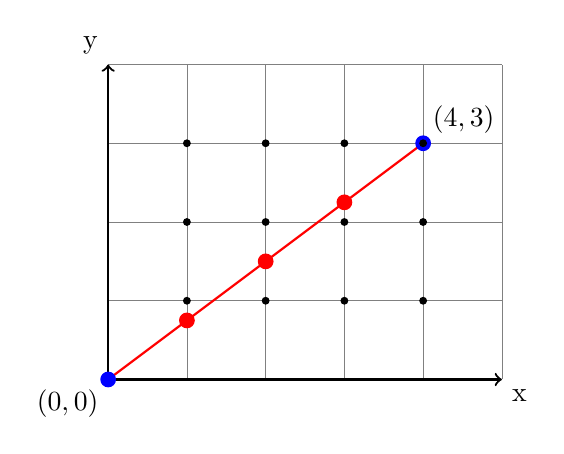
\begin{tikzpicture}[scale=1]
        \draw[step=1cm,gray,very thin] (0,0) grid (5,4);
    
        \draw[thick,->] (0,0) -- (5,0) node[anchor=north west] {x};
        \draw[thick,->] (0,0) -- (0,4) node[anchor=south east] {y};
    
        \draw[thick,red] (0,0) -- (4,3);
    
        \fill[blue] (0,0) circle (0.1);
        \node[below left] at (0,0) {$(0,0)$};
        \fill[blue] (4,3) circle (0.1);
        \node[above right] at (4,3) {$(4,3)$};
    
        \foreach \x in {1,2,3,4} {
            \foreach \y in {1,2,3} {
                \fill[black] (\x,\y) circle (0.05);
            }
        }
    
        \fill[red] (1,0.75) circle (0.1); % (1,0.75)
        \fill[red] (2,1.5) circle (0.1);  % (2,1.5)
        \fill[red] (3,2.25) circle (0.1); % (3,2.25)
    \end{tikzpicture}
\end{center}

\vspace{0.5cm}

次に、$(x, y)$が互いに素ではない場合、つまり最大公約数が1よりも大きい場合を考えます。このとき、$x = g \cdot x', y = g \cdot y'$と表すことができます。$g$が1よりも大きい場合は、
$(0, 0)$と$(x, y)$を結ぶ線分は格子点を通ることがあります。この$(x, y)$を最大公約数$g = 4$で割ると、$(0, 0)$と$(3, 1)$となり、3と1は互いに素です。先ほどのように互いに素の場合は
格子点は存在しません。$d = 4$というのはこの互いに素という格子点の最小単位が4つであることを示しています。今回の設定では、線分の端は格子点に含まれないので、格子点の個数は$4 - 1 = 3$個です。

\vspace{0.5cm}

\begin{center}
    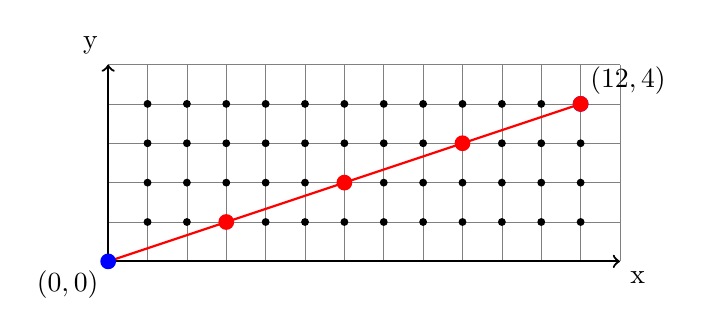
\begin{tikzpicture}[scale=0.5]
        % Draw the grid
        \draw[step=1cm,gray,very thin] (0,0) grid (13,5);
    
        % Draw the x and y axes
        \draw[thick,->] (0,0) -- (13,0) node[anchor=north west] {x};
        \draw[thick,->] (0,0) -- (0,5) node[anchor=south east] {y};
    
        % Draw the line segment from (0,0) to (12,4)
        \draw[thick,red] (0,0) -- (12,4);
    
        % Mark the points (0,0) and (12,4)
        \fill[blue] (0,0) circle (0.2);
        \node[below left] at (0,0) {$(0,0)$};
        \fill[blue] (12,4) circle (0.2);
        \node[above right] at (12,4) {$(12,4)$};
    
        % Mark the grid points around the line segment
        \foreach \x in {1,...,12} {
            \foreach \y in {1,...,4} {
                \fill[black] (\x,\y) circle (0.1);
            }
        }
    
        % Highlight the points that lie on the line segment
        \foreach \i in {3,6,9,12} {
            \fill[red] (\i,{\i/3}) circle (0.2);
        }
    
    \end{tikzpicture}
\end{center}

\vspace{0.5cm}

実装例を以下に示します。

\begin{lstlisting}[caption=2点間の格子点の個数の実装, label=grid, frame=TRBL]
def GCD(a: int, b: int) -> int:
    if a < b:
        a, b = b, a
    if b == 0:
        return a
    
    return GCD(b, a % b)

def count_grid_points(x1: int, y1: int, x2: int, y2: int) -> int:
    x, y = abs(x1 - x2), abs(y1 - y2)
    return GCD(x,y) - 1
\end{lstlisting}

他にも様々な性質があります。

\begin{theorembox}[互いに素と一次不定方程式]
    $a, b \in \mathbb{Z}$が互いに素であるとき、
    \begin{equation*}
        ax + by = 1
    \end{equation*}
    を満たす$x, y \in \mathbb{Z}$が存在する。
\end{theorembox}

これは上で見た拡張ユークリッドの互除法そのものです。

\begin{theorembox}
    $a, b \in \mathbb{Z}$が互いに素であるとき、$b \in \mathbb{Z}$に関して$bc$が$a$で割り切れるなら、
    $c$は$a$の倍数である。

    \textbf{証明}  \\
    $a, b$は互いに素であるから、$ax + by = 1$を満たす$x, y \in \mathbb{Z}$が存在する。
    \begin{equation*}
        c = c \times 1 = c (ax + by) = acx + bcy
    \end{equation*}
    $acx$は自明に$a$で割り切れる。$bcy$も条件より$a$で割り切れるから、$c$は$a$の倍数である。

\end{theorembox}

\begin{theorembox}[合同式の割り算]
    $a, m \in \mathbb{Z}$が互いに素であるとする。
    \begin{equation*}
        ax \equiv by \mod{m}
    \end{equation*}
    であるとき、
    \begin{equation*}
        x\equiv y (\mod{m})
    \end{equation*}
    が成立する。
\end{theorembox}

\begin{theorembox}[倍数の周期性]
    $a, m \in \mathbb{Z}$が互いに素であるとする。
    \begin{equation*}
        0, a, 2a, \cdots, (m - 1)a
    \end{equation*}
    を$m$で割った余りを昇順に並び替えると、$0, 1, 2, \cdots, m - 1$になる。
\end{theorembox}

\begin{theorembox}[逆元と合同方程式]
    $a, m \in \mathbb{Z}$が互いに素であるとする。任意の$b \in \mathbb{Z}$に対して、
    \begin{equation*}
        a x \equiv b \mod{m}
    \end{equation*}
    を満たす$x \in \mathbb{Z}$が$m$を法としてただ一つ在する。特に、$b = 1$の場合を逆元という。
\end{theorembox}

\subsection{中国剰余定理}


\begin{theorembox}[中国剰余定理]
    $n_1, n_2 \in \mathbb{N}$が互いに素であるとき、
    \begin{equation*}
        x \equiv a_1 \mod{n_1}, x \equiv a_2 \mod{n_2}
    \end{equation*}
    を満たす$x$は、$n_1 n_2$を法としてただ一つ存在する。
\end{theorembox}

\begin{theorembox}[Euler関数は乗法的]
\end{theorembox}

\begin{theorembox}[Eulerの定理]
\end{theorembox}

\newpage
\begin{tcolorbox}[enhanced,
    colback=white!85!gray,
    drop fuzzy shadow,
    boxrule=0.3mm,
    arc=0mm,
    left=0pt,
    top=0pt,
    sharp corners,
    width=\textwidth,
    ]
    \textbf{オイラー関数} \\
    オイラー関数とは、自然数$N$が与えられたときに、$1, 2, \cdots, N$のうち$n$と互いに素になる数の個数を求める関数$\Phi(N)$
    です。
  \tcblower
  
  \begin{tcolorbox}[
    coltext=white!10!blue,
    colback=white!90!purple!90!blue,
    drop fuzzy shadow,
    boxrule=0mm,
    arc=0mm,
    width=1.3cm,
    left=0pt,
    right=0pt,
    top=0pt,
    bottom=0pt,
    halign=flush left,
  ]
  \end{tcolorbox}
  \tcblower
  \textbf{回答:}
  \begin{lstlisting}
def enumerate_divisors(n: int) -> list[int]:
    divisors = set()
    for i in range(1, int(n ** 0.5) + 1):
        if n % i == 0:
            divisors.add(i)
            if i != n // i:
                divisors.add(n // i)
    
    return list(divisors)


def main():
    n = int(input())
    divisors = enumerate_divisors(n)
    
    print(*divisors)
    
if __name__ == "__main__":
    main()

  \end{lstlisting}
  \end{tcolorbox}% タイトルの独立

\subsection{問題}

問題1  yukicoder No.442 和と積 \\
2つの整数$a, b$が与えられるので、$a + b, a \times b$の最大公約数を求める問題です。
\begin{lstlisting}[caption=2点間の格子点の個数の実装, label=grid, frame=TRBL]
\end{lstlisting}

\subsection{参考}

\begin{itemize}
    \item \url{https://qiita.com/drken/items/ae02240cd1f8edfc86fd}
\end{itemize}

\section{冪乗: 繰り返し二乗法}

$x^n$を求める際に単に$x \times x \times \cdots \times x$と計算すると$O(n)$の計算量がかかります。繰り返し二乗法を用いると、$O(\log n)$で計算することができます。
また、冪乗では計算結果が非常に大きくなることがあるので、計算結果をmodで割った余りを求めることがあります。剰余で答えを出すときの演算によって処理が異なるので
注意が必要です。

\begin{itemize}
    \item 加算: 加算した後でmodを取る
    \item 減算: 減算した後でmodを取る
    \item 乗算: 乗算した後でmodを取る
    \item 除算: 計算途中でmodを取るときは逆元を用いる(後述)
\end{itemize}

\begin{lstlisting}[caption=繰り返し二乗法の実装, label=power, frame=TRBL]
def exp_mod(n: int, m: int, mod: int) -> int:
    if m == 0:
        return 1
    if m == 1:
        return n % mod
    ans = 1
    m1, m2 = m // 2, m % 2
    ans *= exp_mod(n, m1, mod) % mod
    ans = (ans * ans) % mod
    
    ans *= exp_mod(n, m2, mod)
    ans %= mod
    
    return ans
\end{lstlisting}

\section{逆元とフェルマーの小定理}

% 乗算のmodは計算結果と計算途中でmodを取ると結果が違いことを説明する
除算のmodを取るとき、計算途中でmodをもとった場合と最後にmodを取った場合で結果が異なることがあります。例えば、$a = 20, b = 4, mod = 6$で考えます。

\begin{itemize}
    \item \textbf{計算途中でmodを取る場合:}
    \begin{enumerate}
        \item まず、\( a \) と \( b \) に対してmodを取ります:
        \[
        a \mod m = 20 \mod 6 = 2
        \]
        \[
        b \mod m = 4 \mod 6 = 4
        \]
        \item 次に、得られたmodの値で除算を行い、さらにmodを取ります:
        \[
        \left(\frac{a \mod m}{b \mod m}\right) \mod m = \left(\frac{2}{4}\right) \mod 6
        \]
        通常の整数除算では、これは0(小数は考慮しない)となるため、
        \[
        0 \mod 6 = 0
        \]
        結果は \( 0 \) になります。
    \end{enumerate}

    \item \textbf{最後にmodを取る場合:}
    \begin{enumerate}
        \item まず、\( a \) を \( b \) で割ります:
        \[
        \frac{20}{4} = 5
        \]
        \item 次に、その結果に対してmodを取ります:
        \[
        5 \mod 6 = 5
        \]
    \end{enumerate}
\end{itemize}

除算のmodを求めるときは、計算途中でmodを取ると結果が異なることがあるので、逆元を用いて計算します。

\subsection{フェルマーの小定理と逆元}

除算におけるmodを考えるために\textbf{フェルマーの小定理}と\textbf{逆元}を導入します。

\begin{tcolorbox}[enhanced,title=フェルマーの小定理, 
    attach boxed title to top left, 
    colback=white!95!blue,
    colbacktitle=white!10!blue!50!black,
    drop fuzzy shadow,
    boxrule=0.25mm,
    ]
    $a$は任意の自然数、$m$を素数で$a, m$が互いに素であるとき、以下の式が成り立つ。
    \begin{equation*}
        a^{m-1} \equiv 1 \pmod{m}
    \end{equation*}
  \end{tcolorbox}

\begin{tcolorbox}[enhanced,title=逆元, 
    attach boxed title to top left, 
    colback=white!95!blue,
    colbacktitle=white!10!blue!50!black,
    drop fuzzy shadow,
    boxrule=0.25mm,
    ]
    $m$が素数で、$a$が$m$では割り切れない整数であるとき、以下の式を満たす$x$が[1, m)の範囲で一意に存在する。
    このような$x$を $\pmod m$における$a$の逆元と呼ぶ。
    \begin{equation*}
        a x \equiv 1 \pmod{m}
    \end{equation*}
  \end{tcolorbox}
  ここで、$a^{m-1} \equiv a \times a^{m-2} \equiv 1 \pmod{m}$となるので、$a^{m-2}$が$a$の逆元であることがわかります。以上より以下のことがわかります。

  \vspace{0.5cm}

  \begin{center}
    \textbf{aで割ることは、aの逆元をかけることと等しい}
  \end{center}

\subsection{問題}
逆元を使った問題を解いてみましょう。

  \begin{tcolorbox}[enhanced,
    colback=white!85!gray,
    drop fuzzy shadow,
    boxrule=0.3mm,
    arc=0mm,
    left=0pt,
    top=0pt,
    sharp corners,
    width=\textwidth,
    ]
    \textbf{問題}
    ${}_n \mathrm{C}_k$を998244353で割ったあまりを求めるプログラムを作成せよ。
  \tcblower

  \begin{tcolorbox}[
    coltext=white!10!blue,
    colback=white!90!purple!90!blue,
    drop fuzzy shadow,
    boxrule=0mm,
    arc=0mm,
    width=1.3cm,
    left=0pt,
    right=0pt,
    top=0pt,
    bottom=0pt,
    halign=flush left,
  ]
  \end{tcolorbox}
  \tcblower
  \textbf{回答} 
  ${}_n \mathrm{C}_k = \frac{n!}{(n - k)! k!}$の剰余を求めるます。$\mod$の世界で除算が登場しているので、逆元を用いて計算します。
  乗算するのは$(n - k)!, k!$であることから、これらで割ることは$\mod$の世界では、これらの逆元つまり、それぞれ$(n - k)!^{(DIV-2)}, k!^{(DIV-2)}$をかけることと等しいです。
  \begin{lstlisting}[caption=${}_n \mathrm{C}_k$を求める, label=combination]
DIV = 998244353

def factorial(n: int) -> list[int]:
    memo = [1] * (n + 1)
    for i in range(1, n + 1):
        memo[i] = (memo[i-1] * i) % DIV
    
    return memo

def inverse(n: int) -> int:
    return pow(n, DIV - 2, DIV)

def comb(n: int, k: int, memo: list[int]) -> int:
    return (memo[n] * inverse(memo[k]) * inverse(memo[n-k])) % DIV
 
n, k = map(int, input().split())
memo = factorial(n)
print(comb(n, k, memo) % DIV)
  \end{lstlisting}
  \end{tcolorbox}% 

\end{document}